\begin{center}

\begin{tikzpicture}[x=1cm,y=1cm]
\tikzstyle{line} = [draw, -latex', very thick]
\draw[use as bounding box, anchor = north west,draw=none] (-1,-1) rectangle (5.5+4.5,3.25+2.25);
%\clip (-1,-1) rectangle (10,5.5);
\linespread{0.5}
%\path [draw,very thick,->] (cxe) edge node[above] {cost}  (corig);
\only<1->{\node[anchor =north west] (text) at (-0.5,5.75){\begin{minipage}{10.0cm}
		Basic idea is to create an atomic level represenstation that `knows' about the neighborhood:\\
		\scriptsize  J. Behler. First Principles Neural Network Potentials for Reactive Simulations of Large Molecular and Condensed Systems, \textit{Angew. Chem. Int. Ed.}, 56, 12828, 2017 \normalsize
		\end{minipage}};}
\visible<2->{\node[anchor=west] (im1) at (-0.5,1.5){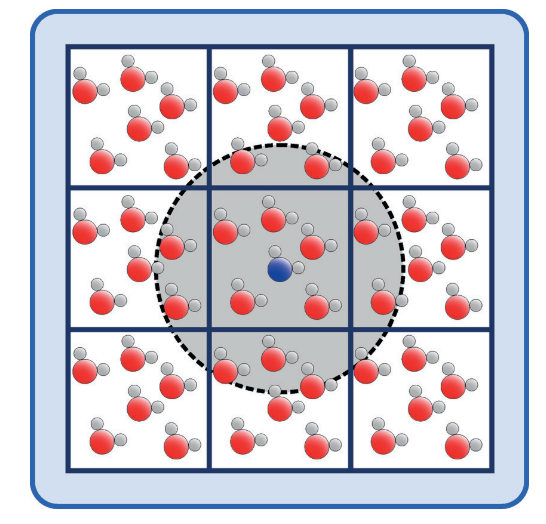
\includegraphics[width=3.5cm]{representations/images/behler-sym-0.png}};}
\visible<3->{\node[anchor=west] (im2) at (5.5,1.5){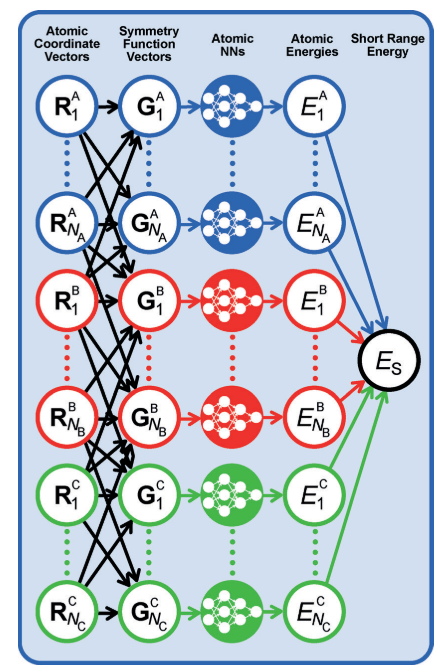
\includegraphics[width=3.15cm]{representations/images/behler-sym-1.png}};}
\visible<3->{\path[draw,blue,ultra thick,->] (im1) -- (im2);}
\visible<4->{\node[anchor =north west, blue] (text) at (-0.5,-0.15){\begin{minipage}{5.5cm}
		\scriptsize  J. Behler and M. Parrinello. Generalized Neural-Network Representation of High-Dimensional Potential-Energy Surfaces, \textit{Phys. Rev. Lett.}, 98, 146401, 2007
		\end{minipage}};}

\end{tikzpicture}

\end{center}
